\chapter{Matériels}

\section{Plateforme mobile} 
\noindent
\begin{tabular}{cc}
 \begin{minipage}{0.5\textwidth} 
 {\large\textbf{Robot Wifibot v2}} \\ \textbf{Dimensions:}\\Hauteur : 18 cm \\ Largeur : 35 cm \\ Longueur : 30 cm \\ Distance entre roues : 0.32 cm \\ Diamètre des roues : 0.18 cm   \end{minipage}
 & 
 \begin{minipage}{0.5\textwidth}
	\begin{figure}[H]
	  \subfloat{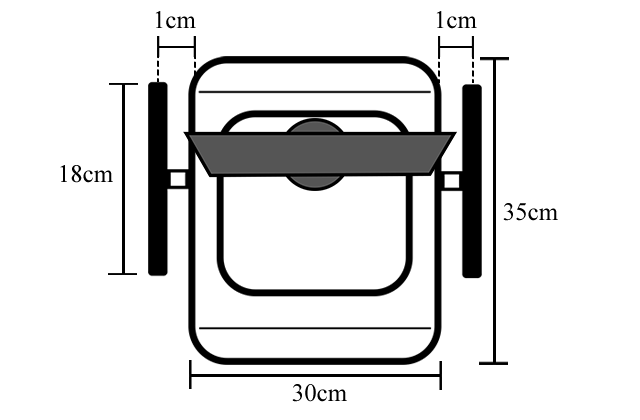
\includegraphics[width=\textwidth]{wbot_mesures.png}}
	\end{figure}
  \end{minipage}
\end{tabular}

\noindent
\begin{tabular}{cc}
\begin{minipage}{0.5\textwidth}  \textbf{Oridnateur portable embarqué :} \\ HD : 8 Go \\ RAM : 2 Go \\ Batterie : 12V NiMH 3.8A 9000mAH \\ Processeur : Intel\textsuperscript{\textregistered} Atom\textsuperscript{TM} N270 @ 1.60GHz \\ Systèm opérationnel : Ubuntu 14.04 \\ Version ROS : ROS Indigo \end{minipage} 
 & 
 \begin{minipage}{0.5\textwidth}
	\begin{figure}[H]
	  \subfloat{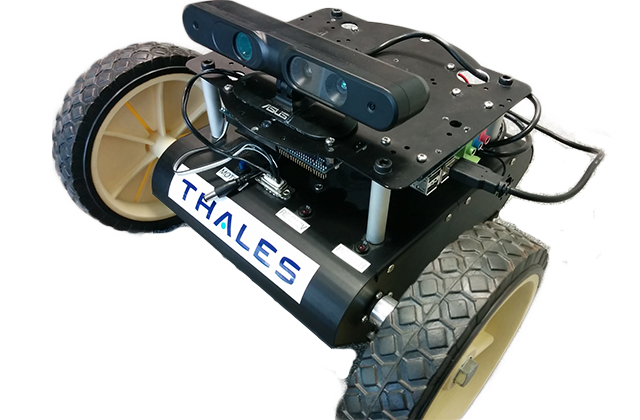
\includegraphics[width=\textwidth]{real_wbot.png}}
	\end{figure}
  \end{minipage}
\end{tabular}



\section{Ordinateur Portable}
\noindent
\begin{tabular}{cc}
\begin{minipage}{0.5\textwidth}
{\large\textbf{HP Pavilion g6}} \\
Processeur :  Intel\textsuperscript{\textregistered} Core\textsuperscript{TM} i5-3230M @ 2.60GHz \\
HD : 750Go \\
RAM : 4Go \\

Systèm opérationnel : Ubuntu 14.04 \\
Version ROS : ROS Indigo \\
\end{minipage}
	 & 
	\begin{minipage}{0.5\textwidth}
		\begin{figure}[H]
		  \subfloat{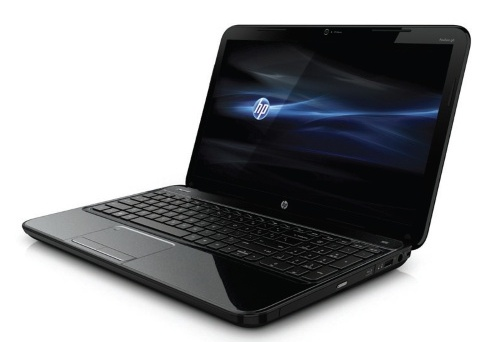
\includegraphics[width=\textwidth]{hp.jpg}}
		\end{figure}
	\end{minipage}
\end{tabular}

% {
%   \raggedleft
%   \begin{tikzpicture} 
%     \node (asus) {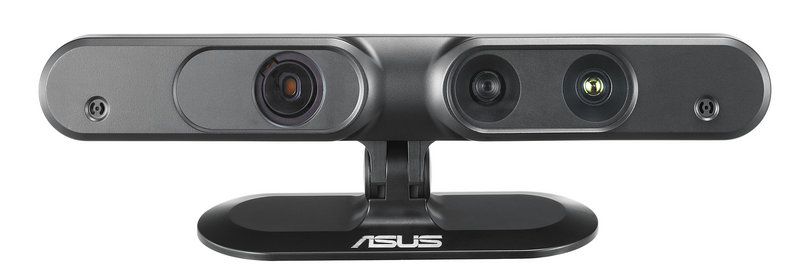
\includegraphics[width=0.4\textwidth]{xtion.jpg}};
%     \node [left=0.5cm of asus.north west, yshift=-5mm]{sdfsf};
%   \end{tikzpicture}
% }

\section{Capteur RGB-D}
\noindent
\begin{tabular}{cc}
	\begin{minipage}{0.5\textwidth} {\large\textbf{Asus Xtion PRO LIVE}} \\
	\textbf{Distance d'utilisation : }\\
	de 0.8 à 3.5 mètres \\
	\textbf{Range de vision : } \\
	58\degree Horizontal, 45\degree Vertical, 70\degree Diagonal \\
	\textbf{Resolution : } \\
	VGA (640x480) : 30 fps \\
	\textbf{Utilisation intérieur}
	\end{minipage}
	 & 
	\begin{minipage}{0.5\textwidth}
		\begin{figure}[H]
		  \subfloat{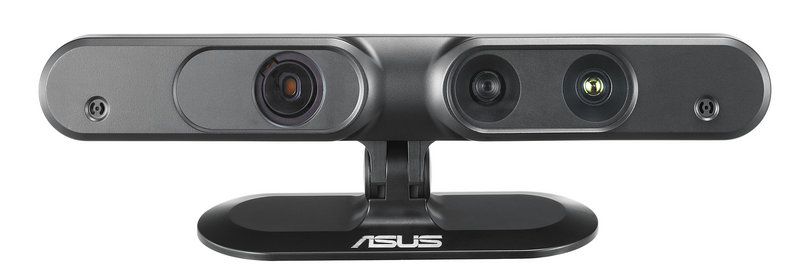
\includegraphics[width=\textwidth]{xtion.jpg}}
		\end{figure}
	\end{minipage}
\end{tabular}


\chapter{Logiciels}

Le design de l'architecture a permis de définir les unités de traitement et la communication entre elles. La définition des unités de traitement suit le découpage du pipeline de reconnaissance avec des nœuds dédiés pour la segmentation, l'extraction de features, la classification, mais également le contrôle du robot.

L'interfaçage matériel-logiciel a été réalisé sur l'environnement ROS - Robot Operating System. En plus d'outils d'affichage, ROS rassemble des librairies d'acquisition d'images RGB-D, OpenNi 2 et Freenect, ainsi qu'une librairie de traitement de nuage de points, PCL.

De plus, sa structure en nœuds a permis une implémentation modulaire et directe du système, ainsi que de gérer la communication entre l'ordinateur portable et le processeur embarqué sur le robot. \\

\url{https://github.com/PointCloudLibrary/pcl/wiki/} \\

\url{http://pointclouds.org/documentation/tutorials/} \\

\chapter{Problèmes rencontrés}

\section{Synchronisation}

La synchronisation entre tous les modules du robot s'est montrée d'extrême importance pour le bon fonctionnement de du système. Retards trop importants résultent en mauvaises transformations de repère, par conséquent, le système de suivi multi-cible n'arrive pas à bien distinguer des objets trop proches. 

\section{Problèmes de déplacement}

La roulette du support originalement installée avait deux axes de
rotation. Pourtant, quelques mouvements de rotation du robot alignent
la roulette orthogonalement au sens du prochain mouvement ce qui crée
un mouvement parasite qui perturbe la trajectoire voulue. Nous avons tenté sans succès d'installer une bille omnidirectionnelle à roulement, qui se
bloquait sur la moquette avec le poids du robot. Une deuxième solution serait d'interdirecertains mouvements du robot pour éviter cette déviation.

\section{Restrictions logicielles}
L' ordinateur embarqué a un puissance de calcul réduite, ce qui ne permet pas que le noeud d'acquisition \(openni2\_launch\) tourne correctment. La solution pour l'instant était de connecter le capteur Asus sur l'ordinateur portable HP.

%\chapter{Evaluation}
%\section{Suivi et reconnaissance multi-cibles}
%\section{Base de données}
%\label{annexe:dataset}
%\begin{figure}[H]
%	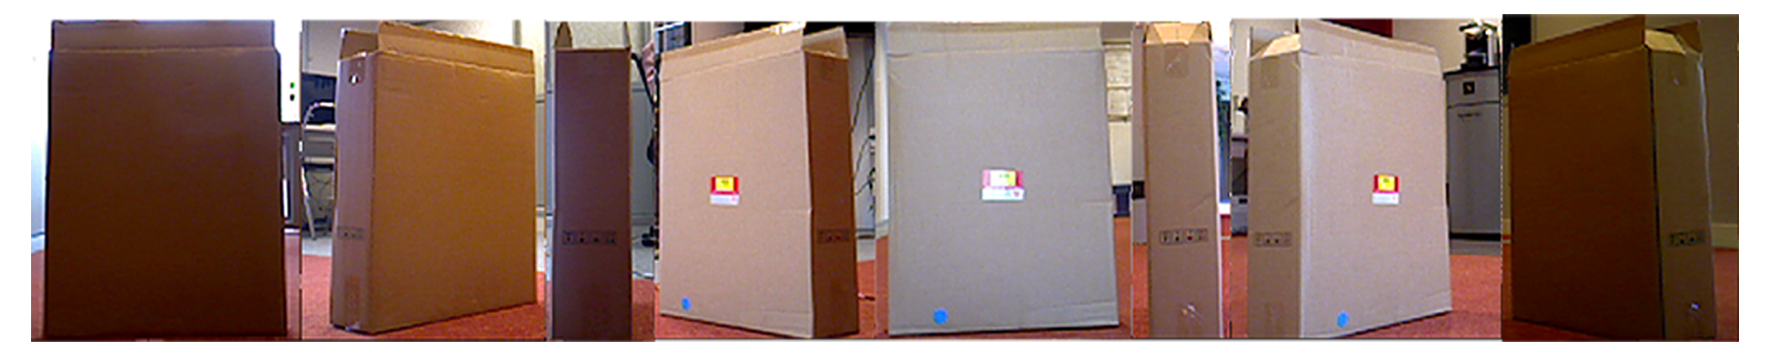
\includegraphics[width=\textwidth]{box_seq.png}
%	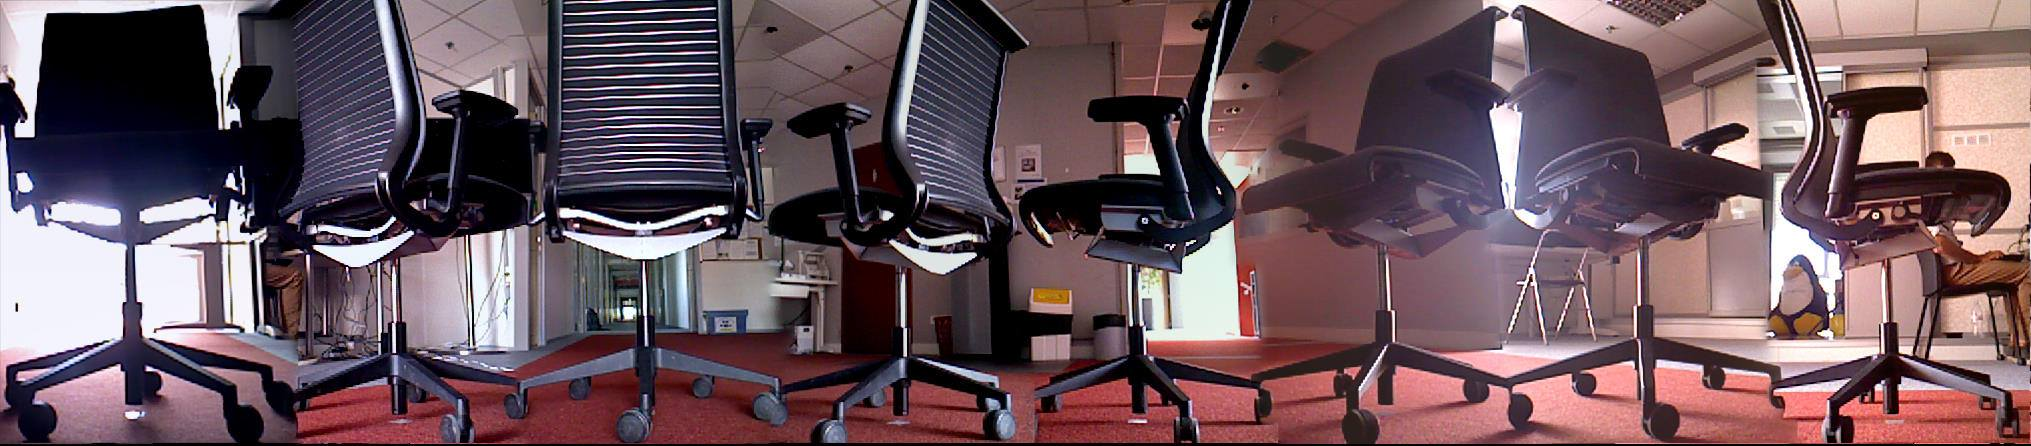
\includegraphics[width=\textwidth]{chair_db.jpg}
%	\label{fig:dataset}
%	\caption{Composition complète de la base de données.}
%\end{figure}
%
%\begin{figure}[H]
 % \subfloat{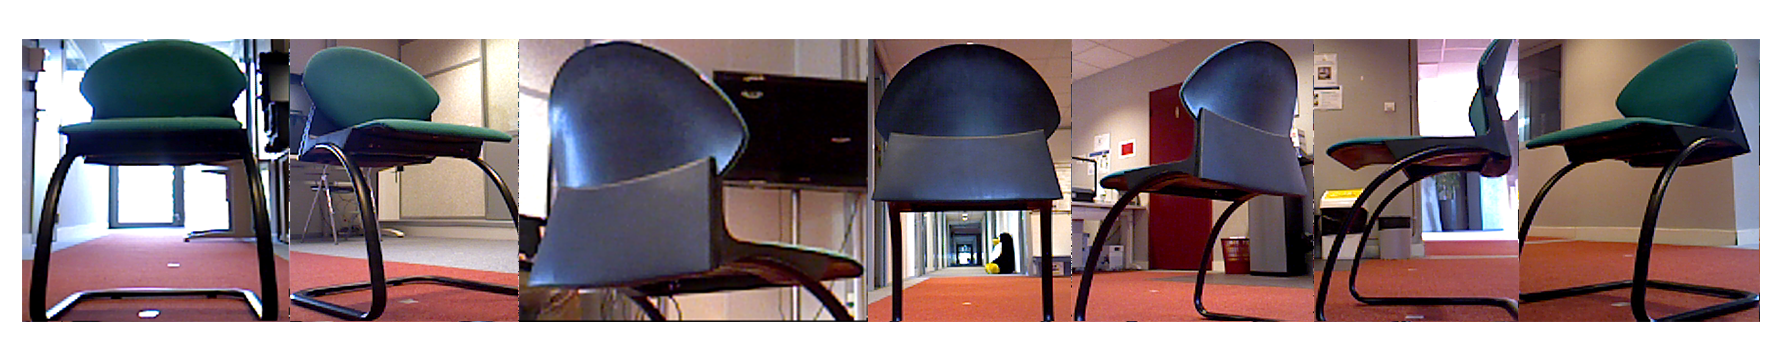
\includegraphics[width=\textwidth]{chair_seq.png}}
%\end{figure}

%\begin{figure}[H]
%  \subfloat{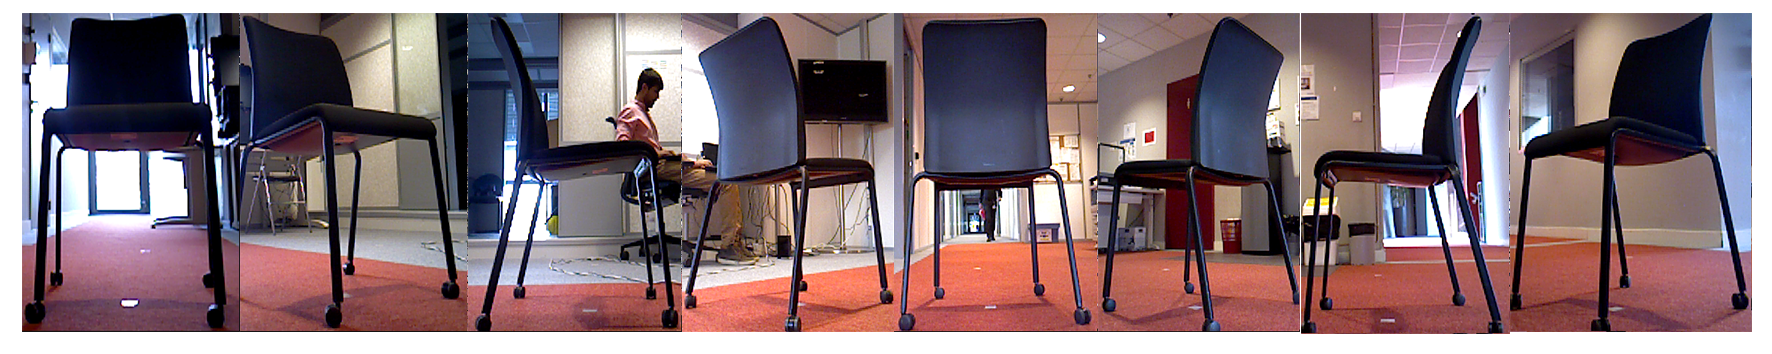
\includegraphics[width=\textwidth]{chair4w.png}}			
%\end{figure}
 
\chapter{Reconnaissance Mono-vue} 
\section{Paramètres Segmentation}
\label{annexe:segmentation}
Le méthode de segmentation exige une définition a priori des paramètres pour le bon fonctionnement du système.
\begin{itemize}
\item Taille du \textit{grid} de voxalization : 2 cm
\item Distance maximale au capteur : 3 m
\item Rayon d'estimation de la normale : 2 cm
\item Aire de \textit{smoothing} de la normale : 10 $cm^2$
\item Distance pour qu'un point soit considéré comme appartenant au plan : 5 cm
\item Distance minimale du plan du sol pour qu'il soit considére comme partie de l'objet : 3 cm
\end{itemize}

La pluparts des valeurs ont été choisies telle qu'elles étaient proposées dans la librarie PCL. Certaines ont été modifiées pour atteindre les caractéristiques attendues.

\section {Descripteurs}
\label{annexe:descripteur}
\subsection{Point Feature Histogram - PFH}

Le PFH utilise les notions de courbure des objets par le calcul de
l'écart entre les normales de points. Ce descripteur peut être calculé
localement ou globalement, en changeant l'importance du rayon de
comparaison. Il est la base d'une grande famille de descripteurs, dont certains seront expliqués par la suite.

En revenant à son calcul, l'histogramme est évalué à partir des paires
de points à l'intérieur d’un ensemble prédéfini. D'abord, un repère
initial, illustré dans l'image \ref{fig:pfh} est établi sachant le vecteur distance normalisé et les normales aux deux points. Ensuite, trois angles, qui correspondent à la transformation angulaire entre les deux normales, et la distance euclidienne entre le deux points sont estimés. Ces quatres valeurs seront considérées comme features pour réduire l’espace initial à douze dimensions - coordonnées et normales des deux point - à un espace à quatre dimensions.


\begin{equation*}
  {\mathsf u} = \boldsymbol{n}_s \qquad
  {\mathsf v} =  {\mathsf u} \times \frac{(\boldsymbol{p}_t-\boldsymbol{p}_s)}{{\|\boldsymbol{p}_t-\boldsymbol{p}_s\|}_{2}}  \qquad
  {\mathsf w} = {\mathsf u} \times {\mathsf v}
\end{equation*}

\begin{figure}[H]
  \centering
  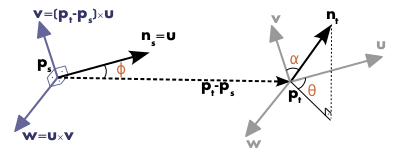
\includegraphics[width=0.6\textwidth]{pfh_frame.png}
  % \caption{{\color{blue} Image d'explication du repère}.}
	\label{fig:pfh}
\end{figure}


Puis, les normales sont transformées en features angulaires décrit par les équations \ref{eq:pfh}
\begin{equation}
  \alpha = {\mathsf v} \cdot \boldsymbol{n}_t  \qquad
  \phi   = {\mathsf u} \cdot \frac{(\boldsymbol{p}_t - \boldsymbol{p}_s)}{d} \qquad
  \theta = \arctan ({\mathsf w} \cdot \boldsymbol{n}_t, {\mathsf u} \cdot \boldsymbol{n}_t) \qquad
  d={\|\boldsymbol{p}_t-\boldsymbol{p}_s\|}_2 
	\label{eq:pfh}
\end{equation}

La prochaine étape est de calculer l'histogramme lui-même. Une
subdivision du range de valeur de chaque feature angulaire, 
normalisés pour rester dans le même intervalle trigonométrique,
est faite et chaque cellule de l'histogramme est incrémenté dès
qu'une feature tombe dans cet intervalle. 

Le PFH est robuste à des différents échelles de densité de points et de bruit, mais aussi invariant à des transformations affines. Ses inconvénients sont liés à la dépendance de la qualité de l'estimation de la normale.

\subsection{Fast Point Feature Histogram - FPFH}

L'utilisation du FPFH vient de la volonté de réduire la complexité du
calcul du descripteur PFH, $ O(nk^2) $, pour un nuage avec $n$ points 
où chacun des points a $k$ voisins . Pour cela, l'algorithme, au
lieu de calculer la relation bidirectionnelle entre tous deux points 
de l’ensemble définis, pondère les features de chaque point  
par les voisins à l'intérieur d'un rayon de recherche, selon la formule
\ref{eq:fpfh}

\begin{equation}FPFH(\boldsymbol{p}_q) = SPFH(\boldsymbol{p}_q) + {1 \over k}
\sum_{i=1}^k {{1 \over \omega_k} \cdot SPFH(\boldsymbol{p}_k)}
\label{eq:fpfh}
\end{equation}

Cette procédure a maintenant une complexité O(n*k). Le gain en vitesse est donc considérable,
ce qui lui permet d'être appliquée pour des utilisations en temps réel. De plus, pour éviter une perte d'information considérable, le FPFH
incorpore quelques point externes au rayon de voisinage, mais qui sont compris dans un rayon de taille donné.

\subsection{Viewpoint Feature Histogram- VFH}

Le VFH, contrairement à PFH et FPFH, est une extension
du deuxième descripteur où la variance de point de vue est prise en
compte. Succintement, des angles entre la normale de chaque point
et la direction principale d'observation sont concaténés à l’histogramme
provenant du SPFH (Simplified PFH). En gardant le repère utilisé dans
les descripteurs précédents, le vecteur de direction principale est défini
par la différence entre l'origine du capteur jusqu'au centroide du
nuage de point considéré. Ce type de feature permet de reconnaitre à la fois
l'objet et son orientation spatiale. Par conséquent, c'est la
feature utilisée dans notre système.

\subsection{Clustered Viewpoint Feature Histogram - CVFH} CVFH -
Clustered VFH - est une feature semi-globale capable de gérer
des occlusions partielles, des erreurs de segmentation et du bruit. Ceci est possible grâce à la
décomposition du \textit{cluster}, segmenté comme objet, en sous-clusters de
structure spatiale homogène. Le descripteur est obtenu d'après un premier
filtrage de zones de fort gradient de courbure, considérés comme zones de
transitions entre surfaces. Puis, l'estimation de l'histogramme VFH pour chaque surface 
donnée par l'algorithme \textit{point growing}. Ainsi, pour un seul objet, le CVFH ne génère pas un seul histogramme VFH, mais un vecteur d'histogrammes.
En revanche, le découpage exige un soin plus important avec la résolution des surfaces afin quelles restent représentatives de l'objet.

\begin{figure}[H]
  \subfloat[PFH ]{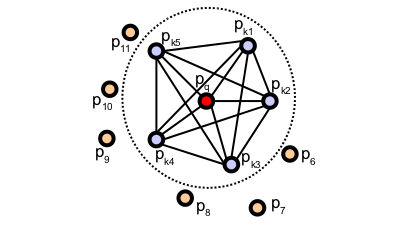
\includegraphics[width=4.5cm]{pfh_diagram.png}}
  \subfloat[FPFH]{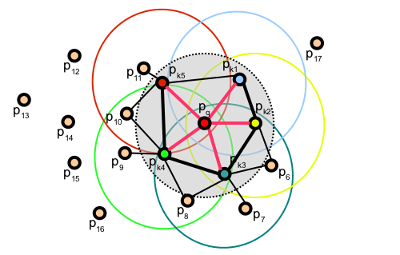
\includegraphics[width=4.5cm]{fpfh_diagram.png}}
  \subfloat[subcaption]{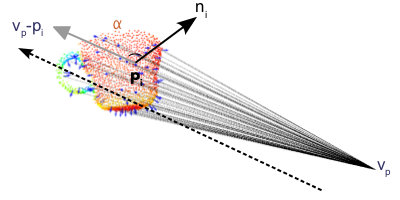
\includegraphics[width=6cm]{second_component.jpg}}		
\end{figure}


\textit{L'Universidad de León } a fait un compte rendu des
\textit{features} implémentés sur PCL dans le lien *[8]*. Plus
d'information sur les descripteur et ses implementations sur la
librarie PCL peuvent être retrouvés sur le site
internet \url{http://pointclouds.org}. \celine{n'oublie pas de mettre un lien}

\subsection{Estimation de la normale}

Pour constituer les informations géométriques l'estimation de la normale du point est d'extrême importance. Sont calcul est fait de la manière suivant :\\
1. Un nombre de voisins est choisi \\
2. Ces point servent à trouver des paramètres de l'équation du plan tangent et, par consequent, la normale correspondent.

Le méthode adopté pour la bibliothéque PCL correspond à prendre un certain nombre de plus proches voisins définis par un seiul. Un petit seil rendre le calcul faux et un grand prend en compte points distants que peuvent ne pas faire partie du plan estimé.\\

\subsection{Déplacement du robot}

Le robot est équipé de trois roues, dont les deux roues symétriques
arrières sont motorisés et responsables du déplacement
moteur. D'autre part, la dernière sert à donner un support pour
la partie arrière du châssis. Les moteurs sont contrôlés à
partir de commandes sériel, préétablis par le fabricant, qui
définissent la vitesse de roulement. La combinaison des rotations
des deux roues motorisées dans les deux sens possibles permets au
robot d'avoir les comportements suivants:

\begin{figure}[H]
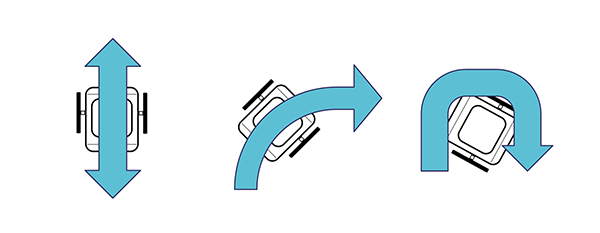
\includegraphics[width=\textwidth]{wbot_mov.png}
\end{figure}
\begin {itemize}
\item Déplacement en ligne droite : deux roues roulant avec la même vitesse et dans le même sens.

\item Déplacement en arc de cercle : différence entre les vitesses des roues.

\item Rotation : deux roues à la même vitesse, mais avec de sens différents.
\end{itemize}

Finalement, la combinaison de ces mouvements permet au robot d'accéder à n'importe quelle position de l’espace.